\section{Структура базового проекта}

\hspace*{0.5cm}Рассмотрим структуру базового проекта. Для этого воспользуемся диаграммой классов UML. Диаграммы классов используются при моделировании программных систем (ПС) наиболее часто. Они являются одной из форм статического описания системы с точки зрения ее проектирования, показывая ее структуру. Диаграмма классов не отображает динамическое поведение объектов изображенных на ней классов. На диаграмме классов показываются классы, интерфейсы и отношения между ними.
\begin{figure}[h!]
\begin{center}
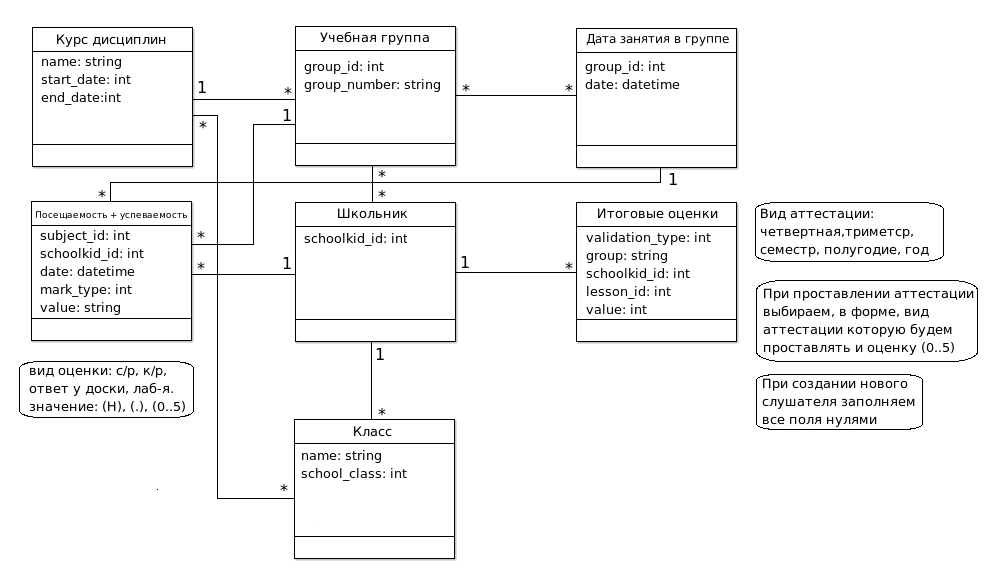
\includegraphics[scale=0.6]{image/class_my.png}
\end{center}
\caption{Диаграмма классов}
\end{figure}
\hspace*{0.5cm}Из данной диаграммы видно, что в системе присутствуют такие классы как:\\
\begin{itemize}
\item курс дисциплин;
\item учебная группа;
\item школьник;
\item посещаемость и успеваемость;
\item дата занятия в группе;
\item класс;
\item итоговые оценки;
\end{itemize}
\hspace*{0.5cm}Класс \textbf{Итоговые оценки} и класс \textbf{Посещаемость и успеваемость} -- классы хранилища, которые содержат информацию об успеваемости и посещаемости слушателей ФДО: оценки, информацию о посещаемости, и т.д. Класс \textbf{Итоговые оценки} находится в отношении один ко многим с классом \textbf{Школьник}.А класс \textbf{Посещаемость и успеваемость} связан отношением один ко многим, с классами \textbf{Школьник}, \textbf{Учебная группа} и \textbf{Дата занятия в группе}. Он содержит информацию о посещаемости и успеваемости слушателя ФДО на данный момент: Оценки и количество посещенных или пропущенных занятий.\\

\section{Разработанные модели}
\hspace*{0.5cm}Для начала определим, какие классы необходимо добавить в систему. Это будут следующие классы:\\
\begin{itemize}
\item \textbf{Школьники} - в этом классе будет храниться информация о школьниках. В этом классе следующие атрибуты: first\_name, second\_name, last\_name, birthday, male, addres, telephone, school\_group\_id, group\_id, created\_at, updated\_at.\\
\item \textbf{Дисциплины} - в данном классе хранится список существующих дисциплин, со следующими атрибутами: full\_name, short\_name, created\_at, updated\_at.\\
\item \textbf{Курсы} - содержит информацию о датах проведения курсов у слушателей ФДО. Имеет следующие атрибуты: start\_date, finish\_date, discipline\_id, created\_at, updated\_at.\\
\item \textbf{Школы} - хранится список школ, из которых поступают абитуриенты. Атрибуты : number, director\_name, director\_surname, director\_pathname, created\_at, updated\_at.\\
\item \textbf{Классы} - данный класс хранит информацию о школьных классах, в которых проходят обучение абитуриенты. Атрибуты : schoolkid\_id, group\_id, created\_at, updated\_at.\\
\item \textbf{Учебные группы} - хранится информация об учебных группа ВУЗа. Данный класс содержит следующие атрибуты : number, year, school\_id, stype, created\_at, updated\_at.\\
\end{itemize}
\endinput
